%!TEX root=../master.tex
%========================================================================================================
% REGRESSION
%========================================================================================================
For \href{https://epfl.ch}{EPFL} \href{https://edu.epfl.ch/coursebook/en/machine-learning-CS-433}{CS433 ML}, \textcopyright \href{https://arnoutdevos.github.io/}{Arnout Devos}
\section{Regression}
\subsection{Linear Regression}
% Simple
% $y_n \approx f(\mathbf{x_n}) := w_0 + w_1 x_{n1}$\newline
% Multiple\newline
$f(\mathbf{x_n}) := w_0 + \sum_{j=1}^D w_j x_{nj} = \tilde{\mathbf{x}}_n^T \mathbf{w}$\newline
If $D > N$ the task is under-determined (more dimensions than data) $\rightarrow$ regularization.

\section{Cost functions}
MSE $= \frac{1}{N} \sum_{n=1}^N [y_n - f(\mathbf{x_n})]^2$ outliers :(\newline
MAE $= \frac{1}{N} \sum_{n=1}^N |y_n - f(\mathbf{x_n})|$\space\space outliers :|\newline
% Error $e_n = y_n - f(\mathbf{x_n})$
\subsection{Convexity}
% A line joining two points never intersects with the function anywhere else.
$f(\lambda \mathbf{u} + (1-\lambda)\mathbf{v}) \le \lambda f(\mathbf{u}) + (1-\lambda) f(\mathbf{v})$ with $\lambda \in [0;1]$ and $u,v\in$convex set$\mathcal{C}$.
\textit{Strictly} convex function: unique global minimum $w^*$. 
% Sums of convex functions are convex. 
Function always above its linearization: \newline $\mathcal{L}(u) \ge \mathcal{L}(w) + \nabla \mathcal{L}(w)^T (u-w) \forall u,w$.

Set is convex iff line between any two points of $\mathcal{C}$ lies in $\mathcal{C}$ : $\theta u + (1 - \theta) v \in \mathcal{C}$

%========================================================================================================
% OPTIM
%========================================================================================================
\section{Optimization}
% Find $\mathbf{w^*} \in \mathcal{R}^D$ which $min\,\,\mathcal{L}(\mathbf{w})$.\newline
Gradient $\nabla \mathcal{L} := \begin{bmatrix} \frac{\partial \mathcal{L}(\mathbf{w})}{\partial w_1} & \dots & \frac{\partial \mathcal{L}(\mathbf{w})}{\partial w_D} \end{bmatrix}$
\subsection{Grid Search $\mathcal{O}(\prod_{i=1}^D|W|_i\times N)$}
no guarantee (local) optimum close
\subsection{Gradient descent $\mathcal{O}(N\times D)$}

$\mathbf{w^{(t+1)}} = \mathbf{w^{(t)}} - \gamma \nabla \mathcal{L}(\mathbf{w^{(t)}})$. ill-cond :(

GD - Linear Regression MSE

$\mathcal{L}(\mathbf{w}) = \frac{1}{2N} (\mathbf{y} - X\mathbf{w})^T(\mathbf{y} - X\mathbf{w}) \rightarrow$ \newline $ \nabla \mathcal{L}(\mathbf{w}) = - \frac{1}{N} X^T(\mathbf{y} - X\mathbf{w})$. Cost: \newline $O_{err} = 2ND + N$ and $O_{w} = 2ND + D$.

\subsection{SGD $\mathcal{O}(D)$}

$\mathcal{L} = \frac{1}{N} \sum_{n=1}^N{\mathcal{L}}_n(\mathbf{w})$ with update \newline $\mathbf{w}^{(t+1)} = \mathbf{w}^{(t)} - \gamma \nabla \mathcal{L}_n(\mathbf{w}^{(t)})$.

\subsection{Mini-batch SGD $\mathcal{O}(|B|\times D)$}

$\mathbf{g} = \frac{1}{|B|} \sum_{n\in B}{\nabla \mathcal{L}}_n(\mathbf{w}^{(t)})$ with update \newline $\mathbf{w}^{(t+1)} = \mathbf{w}^{(t)} - \gamma \mathbf{g}$.

\subsection{Subgradient at $w$}

$\mathbf{g} \in \mathbb{R}^D$ with $\mathcal{L}(u) \ge \mathcal{L}(w) + \mathbf{g}^T (u-w)$. 

% Example subgradient for MAE: $h(e) = |e| \rightarrow g(e) = {sgn(e) \text{ if } e \ne 0, \lambda \in [-1;1] \text{ otherwise }}$. We get the gradient:\newline $\nabla \mathcal{L}_{MAE} = - \frac{1}{N} \sum_n sgn(y-f(x_n)) \nabla f(x_n)$.

\subsection{Projected SGD $\mathcal{P_C}(w')=\arg\min_{v\in\mathcal{C}}\norm{v-w'}$}

$\mathbf{w}^{(t+1)} = \mathcal{P_C} [\mathbf{w}^{(t)} - \gamma \nabla \mathcal{L}(\mathbf{w}^{(t)})]$

\subsection{Newton's method $\mathcal{O}(ND^2 + D^3)$}\label{Newton}
2nd order, !cheap, faster convergence

$w^{(t+1)} = w^{(t)} - \gamma^{(t)} (H^{(t)})^{-1} \nabla \mathcal{L}(w^{(t)})$

\subsection{Optimality conditions}
Necessary: $\nabla \mathcal{L} (\mathbf{w}^*) = 0$,
Sufficient: Hessian PSD $\mathbf{H}(\mathbf{w}^*) := \frac{\partial^2 \mathcal{L}(\mathbf{w}^*)}{\partial w \partial w^T}$
\newline
%========================================================================================================
% LEAST SQUARES
%========================================================================================================

\section{Least Squares}
\subsection{Normal Equation}
$X^T (\mathbf{y} - X\mathbf{w})= 0 \Rightarrow$\newline$\mathbf{w^*} = (X^TX)^{-1}X^T\mathbf{y} \text{ and } \mathbf{\hat{y}_m} = \mathbf{x_m^T} \mathbf{w^*}$
Gram matrix $\in \mathbb{R}^{D\times D}$ invertible iff $rank(X) = D$ (else use $X = USV^T \in \mathbb{R}^{N\times D}$ to get pseudo-inverse $\mathbf{w^*} = V\tilde{S}U^Ty$ with $\tilde{S}$ pseudo-inverse of $S$: $\tilde{\sigma_i} = 1/\sigma_i, \forall \sigma_i \ne 0$). cost$(A^{-1})=\mathcal{O}(N^3)$

\section{Likelihood}
Probabilistic model $y_n = \mathbf{x_n}^T\mathbf{w} + \epsilon_n$.
Probability of observing the data given a set of parameters + inputs:
$p(\mathbf{y}|X, \mathbf{w}) = \prod_n p(y_n|\mathbf{x_n}, \mathbf{w})  = \prod_n \mathcal{N} (y_n | \mathbf{x_n}^T\mathbf{w}, \sigma^2)$

Maximizing log-likelihood (=$min_w$ MSE) $\mathcal{L}_{LL} = -\frac{1}{2\sigma^2} \sum(y_n-x_n^Tw)^2+cst$.


%========================================================================================================
% REGULARISATION
%========================================================================================================
\section{Regularization}
\subsection{Ridge Regression $\mathcal{O}(D^3+ND^2)$}
$\mathcal{L}(\mathbf{w}) = \frac{1}{2N} (\mathbf{y} - X\mathbf{w})^T(\mathbf{y} - X\mathbf{w}) + \frac{\lambda}{2} ||\mathbf{w}||^2_2 \rightarrow$
$\mathbf{w^*_{ridge}} = (X^TX + 2N\lambda I)^{-1}X^T\mathbf{y}$\newline

Can be considered a MAP estimator : $\mathbf{w^*_{ridge}} = arg min_w - log(p(w|X,y))$

\subsection{Lasso regularizer}
Sparse solution.
$\mathcal{L}(w) = \frac{1}{2N} (y - Xw)^T(y - Xw) + \lambda ||w||_1 $

%========================================================================================================
% MODEL SELECTION
%========================================================================================================
\section{Model Selection, eg crossval $\rightarrow\lambda$}
$P\left[|L_\mathcal{D}-L_{S_{test}}|)\ge \sqrt{\frac{(b-a)^2ln(2/\delta)}{2|S_{test}|}}\right]\leq \delta$ More data points ($|S_{test}|\uparrow$) =  more confident close to true loss. $a\leq L\leq b$
\subsection{Bias-Variance = vary train data}
Small dim: large bias, small var.
Large dim: small bias, large var.
Error for the val set compared to the emp distr of the data $\propto \sfrac{\sqrt{ln(|\Omega|)}}{\sqrt{|V|}}$.


%========================================================================================================
% CLASSIFICATION
%========================================================================================================
\section{Classification}
\subsection{Optimal}
$\hat{y}(\mathbf{x}) = argmax_{y\in \mathcal{Y}} p(y|\mathbf{x})$

\subsection{Logistic regression}\label{logreg}
$\sigma(z) = \frac{e^z}{1+e^z}$ to limit the predicted values $y\in [0;1]$ ($p(1|\mathbf{x}) = \sigma(\mathbf{x}^T\mathbf{w})$ and $p(0|\mathbf{x}) = 1-\sigma(\mathbf{x}^T\mathbf{w})$). Decision wrt $0.5$.

Likelihood

$p(y | X,w) = \prod p(y_n|x_n) \newline =\underset{n:y_n=0}{\prod} p(0|x_n) \dots \underset{n:y_n=K}{\prod} p(K|x_n) \newline = \prod_k \prod_n [p(y_n = k | x_n,w)]^{\tilde{y}_{nk}}$ \newline where ${\tilde{y}_{nk}} = 1$ if $y_n=k$.

For binary classification

$p(y | X, w) = \underset{n:y_n=0}{\prod} p(0|x_n) \dots\underset{n:y_n=1}{\prod} p(1|x_n) \newline = \underset{n}{\prod} \sigma({x_n^T w})^{y_n}[1-\sigma({x_n^T w})]^{1-y_n}$

Loss

$\mathcal{L}(w) = \sum_{n=1}^N ln(1 + exp(x_n^T w)) - y_n x_n^T w$ which is convex in $w$.

Gradient

$\nabla \mathcal{L}(w) = \sum_{n=1}^N x_n (\sigma(x_n^T w) - y_n) = X^T[\sigma(Xw) - y]$ (no closed-form).

 Hessian $H(w) = X^T S X$, $S_{nn} = \sigma(x_n^T w)[1-\sigma(x_n^T w)]$ (cvx/Newton \ref{Newton}).
If data lin sep: $w*\rightarrow\infty$ so regularize
\subsection{Exponential family}
General form

$p(y|\eta) = h(y) exp[\boldsymbol{\eta}^T \boldsymbol{\phi}(y) - A(\boldsymbol{\eta})]$

Cumulant

$A(\eta) = ln[\int_y h(y) exp[\eta^T \phi(y)] dy]$
\newline
$\nabla A(\eta) = \mathbb{E}[\phi(y)] = \mu = g^{-1}(\eta)$
\newline
$\nabla^2 A(\eta) = \mathbb{E}[\phi\phi^T] - \mathbb{E}[\phi]\mathbb{E}[\phi^T]$

Link function

$\eta = g(\mu) \Leftrightarrow \mu = g^{-1}(\eta)$

$\eta_{gaussian} = (\sfrac{\mu}{\sigma^2}, -\sfrac{1}{2 \sigma^2})$
; $\eta_{poisson} = ln(\mu)$
; $\eta_{bernoulli} = ln(\sfrac{\mu}{1 - \mu})$
\newline $\eta_{general} = g^{-1}(\frac{1}{N} \sum_{n=1}^N \phi(y_n))$

GLM: scalar $\phi(y)$, $\eta_n=\boldsymbol{x}_n^T\boldsymbol{w}$, see \ref{logreg}

$\nabla_w \mathcal{L}(w)= X^T [g^{-1}(Xw)- \phi(y)]= 0$

\subsection{Nearest Neighbor, best low dim}
\subsubsection{k-NN}
$f_{S^{tr,k}}(x) = \frac{1}{k} \sum_{n:x_n\in nbh_{S{tr,k}(x)}} y_n$.
Pick odd $k$ so clear winner.
Large $k \rightarrow$ large bias + small variance (inv.)

Error bound, opt Bayes $f^*$

$\mathbb{E}[\mathcal{L}_{St}] \le 2 \mathcal{L}_{f^*} + 4 c \sqrt{d} N^{-1/d+1}$

Curse: cst Loss: $N=(1/\alpha)^{d+1}, \alpha << 1$

\subsection{Support Vector Machines (SVM)}
Logistic regression with hinge loss :
$min_w \sum_{n=1}^N [1-y_n x_n^T w]_+ + \frac{\lambda}{2} ||w||^2$ where $y \in [-1;1]$ the label and $hinge(x)= max\{0,x\}$. Convex but not differentiable so need subgradient.

Duality: $\mathcal{L}(w) = max_{\alpha} G(w, \alpha)$. Primal SVM 
$min_{w} max_{\alpha \in [0,1]^N} \sum \alpha_n (1 - y_nx_n^Tw) + \sfrac{\lambda}{2} ||w||^2$ is diff + cvx. Can switch (=dual) $max$ and $min$ when convex in $w$ and concave in $\alpha$. Simpler form:\newline
$w(\alpha) = \frac{1}{\lambda} \sum \alpha_n y_n x_n = \frac{1}{\lambda} X^T diag(y) \alpha$ which plugging into primal yields:\newline
$max_{\alpha \in [0,1]^N} \alpha^T\mathbf{1} - \sfrac{1}{2\lambda} \alpha^T Y X X^T Y \alpha$\newline


The solution is sparse ($\alpha_n = 0$ correct side,$\alpha_n \in (0,1)$ on margin, $\alpha_n =1$ inside margin/wrong side). Coord ascent on $\boldsymbol{\alpha}_n$

\subsection{Kernel Ridge Regression}
From duality $w^* := X^T \alpha^*$ where $\alpha^* := (K + \lambda I_N)^{-1}y$ and $K=XX^T = \phi^T(x) \phi(x) = \kappa(x,x')$ (needs to be PSD and symmetric). $\mathcal{O}(N^3+DN^2)$


%========================================================================================================
% UNSUPERVISED LEARNING
%========================================================================================================
\section{Unsupervised Learning}
\subsection{K-means clustering}

$min\,\,\mathcal{L}(z,\mu) = \sum_n^N \sum_k^K z_{nk} ||x_n - \mu_k||^2_2$ with $z_{nk} \in \{0,1\}$ (unique assignments: $\sum_k z_{nk} = 1$).

Algorithm (Coordinate Descent $z$, $\mu$)

1. $\forall n,$ $z_n = \begin{cases}
	1 \text{ if } k = argmin_j || x_n - \mu_j||^2 \\
	0 \text{ otherwise }
   \end{cases}$
2. $\forall k$ compute $\mu_k = \sfrac{\sum_n z_{nk} x_n}{\sum_n z_{nk}}$

Probs:cost,spher+hard clusters

Probabilistic model

$p(X|\mu,z) = \underset{n}{\prod}  \mathcal{N}(x_n|\mu_k,I) \newline= \underset{n}{\prod} \underset{k}{\prod}  \mathcal{N}(x_n|\mu_k,I)^{z_{nk}}$

\subsection{Gaussian Mixture Models}
$p(X,z|\mu,\Sigma,\pi) = \underset{n}{\prod} (x_n|z_n,\mu_k,\Sigma_k)p(z_n|\pi)
= \underset{n}{\prod}\underset{k}{\prod} [\mathcal{N}(x_n|\mu_k,\Sigma_k)]^{z_{nk}} \underset{k}{\prod} [\pi_k]^{z_{nk}}$ \newline where $\pi_k = p(z_n=k)$

Marginal likelihood: $z_n$ latent variables => factored out of likelihood \newline $p(x_n|\theta) = \sum_k \pi_k \mathcal{N}(x_n|\mu_k, \Sigma_k)$.\newline nb params with $z$ (D,K<<N): $\mathcal{O}(N)$, marg out $z$: $\mathcal{O}(D^2K)$.

\subsection{EM}
\subsubsection{GMM}
Intialize $\mu^{(0)}, \Sigma^{(0)}, \pi^{(0)}$.

1. E-step: Compute the assignments. $q_{kn}^{(t)} := \frac{\pi_k^{(t)} \mathcal{N}(x_n|\mu_k^{(t)}, \Sigma_k^{(t)})}{ \sum_k^K\pi_k^{(t)} \mathcal{N}(x_n|\mu_k^{(t)}, \Sigma_k^{(t)}) }$
(2. Compute Marginal Likelihood)
3. M-step: Update

$\mu_k^{(t+1)} = \frac{\underset{n}{\sum} q_{nk}^{(t)} x_n}{\underset{n}{\sum} q_{nk}^{(t)}}$ $\pi_k^{(t+1)} = \frac{1}{N} \underset{n}{\sum} q_{nk}^{(t)}$

$\Sigma_k^{(t+1)} = \frac{\underset{n}{\sum} q_{nk}^{(t)}(x_n - \mu^{(t+1)})(x_n - \mu^{(t+1)})^T}{\underset{n}{\sum} q_{nk}^{(t)}}$
\newline

\subsubsection{General}
$\theta^{(t+1)} := argmax_{\theta} \underset{n}{\sum} \mathbb{E}_{p(z_n|x_n,\theta^{(t)})}\newline[log\,\, p(x_n,z_n|\theta)]$\newline

%========================================================================================================
% Matrix Factorizations
%========================================================================================================
\section{Matrix Factorisations}
\subsection{Prediction}
Find $\mathbf{X} \approx \mathbf{W}\mathbf{Z}^T$ where $\mathbf{W} \in \mathbb{R}^{D\times K}$ and $\mathbf{Z} \in \mathbb{R}^{N\times K}$ with $K << D,N$. Large $K\rightarrow$ overfitting. If $K \ge max\{D,N\}$ trivial solution ($W=\mathbf{1}_D$ or $Z=\mathbf{1}_N$).

Quality of reconstruction (not jointly convex nor identifiable):\newline $\mathcal{L}(\mathbf{W}, \mathbf{Z}) := \frac{1}{2} \underset{(d,n)\in \Omega}{\sum} [x_{dn} - (\mathbf{W}\mathbf{Z}^T)_{dn}]^2 \newline= \underset{(d,n)\in \Omega}{\sum} f_{dn}(w,z)$

Regularizer: $\frac{\lambda_w}{2} ||\mathbf{W}||^2_{Frob} + \frac{\lambda_z}{2} ||\mathbf{Z}||^2_{Frob}$

Opt SGD ($\nabla_{w_{d'k}}$ for fixed user $d'$ and $\nabla_{z_{n'k}}$ for fixed item $n'$, $=[x_{dn}-(\mathbf{W}\mathbf{Z}^T)_{dn}]\{z_{nk} (d'=d)), w_{dk} (n'=n))\} $) . 

ALS (assume no missing ratings):

$\mathbf{Z}^T_* = (\mathbf{W}^T\mathbf{W} + \lambda_z I_K)^{-1} \mathbf{W}^T \mathbf{X}$

$\mathbf{W}^T_* = (\mathbf{Z}^T\mathbf{Z} + \lambda_w I_K)^{-1} \mathbf{Z} \mathbf{X}^T$
\subsection{Text Representation}
MF of co-occurence $X$: row($\mathbf{W}$) is wordvec, row($\mathbf{Z}$) is \textit{context} wordvec.
\textbf{GloVe}
$f_{dn} = min\{1,(\frac{n_{dn}}{n_{max}})^\alpha\}, \alpha \in [0;1]$ weighted loss factors. Train as MF.

Skipgram/CBOW, f(.) context/word
Bin classif to real/fake word pairs.
\subsection{FastText superv $f(y_nWZ^Tx_n)$}
Doc-Sent, BoW, $x_n\in\mathbb{R}^{|V|}$=sent, f lin
%========================================================================================================
% DIM RED
%========================================================================================================
\section{Dimensionality reduction}
\subsection{SVD (no missing entries)}
$\mathbf{X} = \mathbf{U} \mathbf{S} \mathbf{V}^T$, with $\mathbf{X}: D\times N$, ($\mathbf{U}: D\times D$, $\mathbf{V}: N\times N$) orthonormal, $\mathbf{S}: D\times N$ diag PSD, $s_i$ in desc ord ($s_1 \ge \dots \ge s_D \ge 0$).

Reconstruction\newline $||\mathbf{X}-\mathbf{\hat{X}}||_F^2 \ge ||\mathbf{X}-\mathbf{U}_K\mathbf{U}_K^T\mathbf{X}||_F^2 = \underset{i\ge K+1}{\sum} s_i^2$ 
\newline$\forall$ rank-$K$ matrix $\mathbf{\hat{X}}$ (i.e. \textit{compress data by project onto left sing vectors.})

Truncated SVD: $\mathbf{U}_K \mathbf{U}_K^T \mathbf{X} = \mathbf{U} \mathbf{S}_K \mathbf{V}^T$

Application to MF: $\mathbf{U} = \mathbf{W}$, $\mathbf{S}\mathbf{V}^T = \mathbf{Z}^T$. Rec. limited by the rank-K of W,Z.

\subsection{PCA = rank-K SVD}
Decorrelate the data. Empirical cov before: $N\mathbf{K} = \mathbf{X}\mathbf{X}^T = \mathbf{U}\mathbf{S}_D^2\mathbf{U}^T$.
After $\mathbf{\tilde{X}} = \mathbf{U}^T\mathbf{X}$: $N\mathbf{\tilde{K}} = \mathbf{\tilde{X}}\mathbf{\tilde{X}}^T = \mathbf{S}_D^2$ (pure diag = components are uncorrelated).

Pitfalls: not invariant under scalings.

%========================================================================================================
% Neural nets
%========================================================================================================
\section{Neural Networks}
The output at the node $j$ in layer $l$ is $x_j^{(l)} = \phi \big(\sum_i w_{i,j}^{(l)}x_i^{(l-1)} + b_j^{(l)} \big)$
\subsection{Representation power 1 layer}
Error $\le \frac{(2Cr)^2}{n}$ where $C$ smoothness bound, $n$ \#nodes. Approx any sufficiently smooth 2D func on bounded domain (\textit{on avg} $\sigma$ act, \textit{pointw} ReLU).
\subsection{Learning}
Problem not convex, but SGD stable. Backpropagation:
Let $\mathcal{L}_n = (y_n - f^{(L+1)} \circ \dots \circ f^{(1)}(\mathbf{x}^{(0)}_n))^2$.\newline
\textbf{Forward pass} \newline $\mathbf{x}^{(0)}=\mathbf{x}_n$. For $l=1,\dots,L+1$ \newline
$\mathbf{z}^{(l)} = (\mathbf{W}^{(l)})^T\mathbf{x}^{(l-1)}+\mathbf{b}^{(l)}$, $\mathbf{x}^{(l)} = \phi(\mathbf{z}^{(l)})$\newline
\textbf{Backward pass} \newline $\delta^{(L+1)} = -2(y_n-\mathbf{x}^{(L+1)})\phi^{'}(\mathbf{z}^{(L+1)})$ and $\forall l$ :
$\delta^{(l)} = (\mathbf{W}^{(l+1)}\delta^{(l+1)}) \odot \phi^{'}(\mathbf{z}^{(l)})$ \newline

\textbf{Final pass} \newline
$\frac{\partial{\mathcal{L}}_n}{\partial w_{i,j}^{(l)}} = \delta^{(l)}_j \mathbf{x}_i^{(l-1)}$, $\frac{\partial{\mathcal{L}}_n}{\partial b_{j}^{(l)}} = \delta_j^{(l)}$, $\delta_j^{(l)}=\frac{\partial{\mathcal{L}}_n}{\partial z_{j}^{(l)}}$

\subsection{Activations}
sigmoid $\phi(x) = 1/(1+e^{-x})= 1 -\sigma(x)$, tanh $\frac{e^x+e^{-x}}{e^x+e^{-x}} = 2 \phi(2x)-1$, ReLU, Leaky ReLU ($max\{\alpha x, x\}$).

\subsection{Convolutional Neural Nets}
Filter $f$: $x^{(1)}[n,m] = \sum_{k,l} f[k,l]x^{(0)}[n-k, m-l]$. Filter local so no fully connected. Same filter at every position: \textit{weight sharing}. Learning: backprop different weights, sum grads shared weights.  Per layer $k<<<K$: params $\mathcal{O}(kK)=\mathcal{O}(K)$ \textit{else} FFT $\mathcal{O}(L\log(L), L\geq N+K-1$

\subsection{Overfitting}
Adding regularization equivalent to weight decay (by $(1-\eta\lambda)$). Can also use dataset augmentation, dropout.


%========================================================================================================
% Graphical models
%========================================================================================================
\section{Graphical Models}
\subsection{Bayes Nets}
$p(X_1,\dots,X_D) = p(X_1)p(X_2|X_1)\dots\newline p(X_D|X_1,\dots,X_{D-1})$. Node is random variable, directed edge from $X_j$ to $X_i$ if $X_j$ appears in the conditioning $p(X_i|\dots,X_j,\dots)$. Graph \textit{acyclic} (must).

Conditional independence: $p(X,Y)=p(X)p(Y)$ or given $Z$ $p(X,Y|Z)=p(X|Z)p(Y|Z)$.

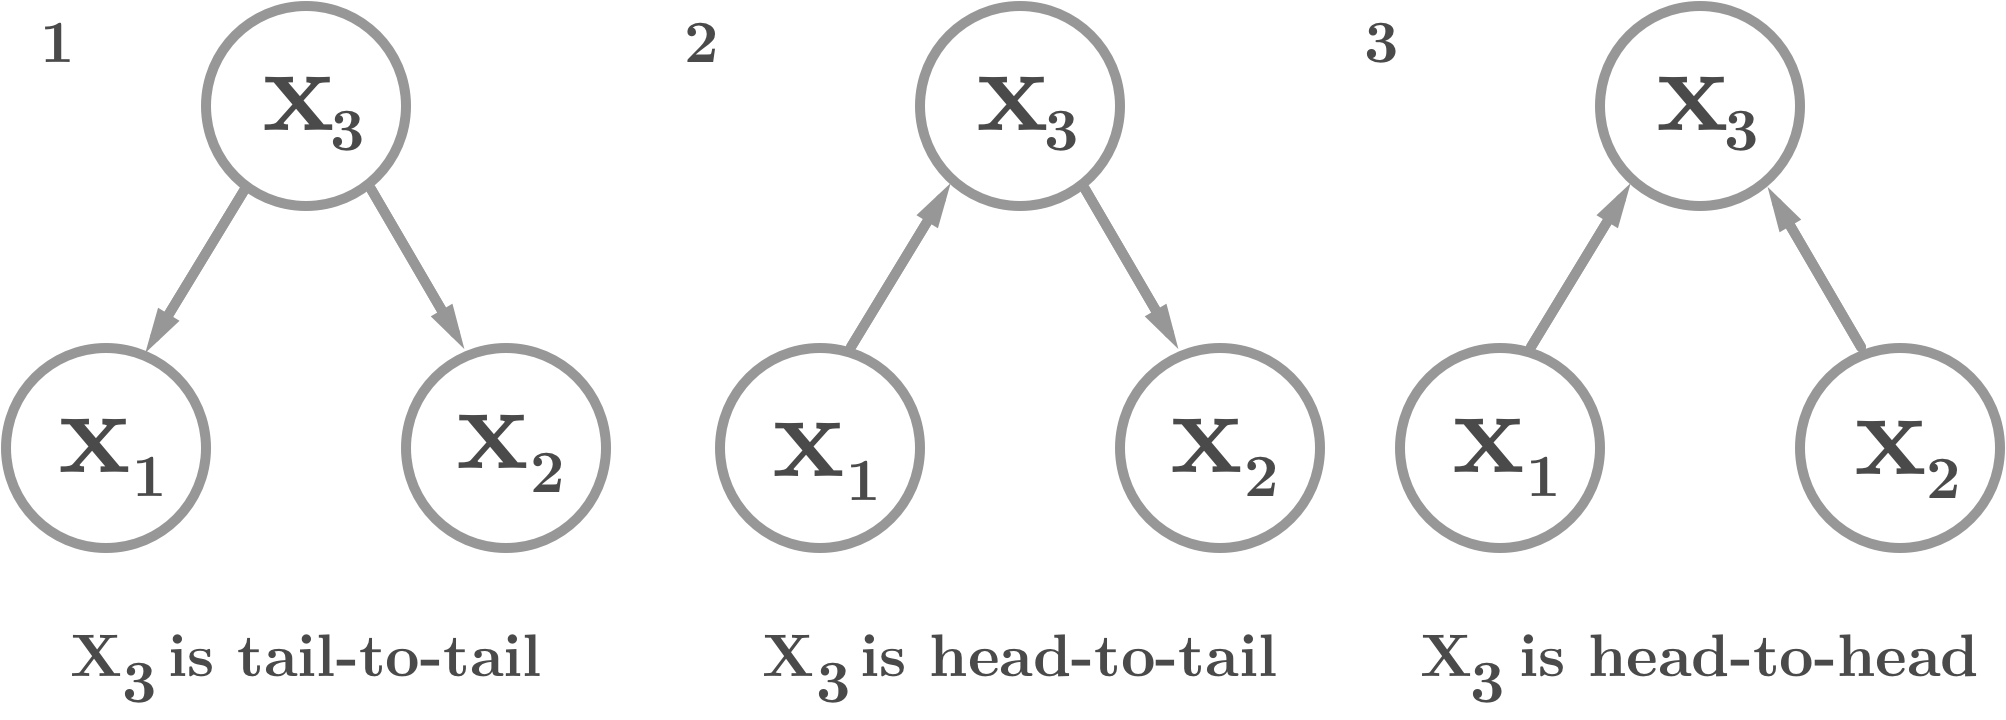
\includegraphics[width=\linewidth]{figs/bayes.png}
1. $p(x_1, x_2, x_3) = p(x_3)p(x_1|x_3)p(x_2|x_3)$ : $x_1$ and $x_2$  indep. given $x_3$\newline
2. $p = p(x_1)p(x_3|x_1)p(x_2|x_3)$ : id.\newline
3. $p = p(x_1)p(x_2)p(x_3|x_1, x_2)$ : $x_1$ and $x_2$  \textbf{not} indep. given $x_3$

$X \rightarrow Y$ path blocked by $Z$ if it contains a variable such that either
1. variable is in $Z$ and it is head-to-tail or tail-to-tail.
2. node is head-to-head and neither this node nor any of its descendants are in $Z$.

$X$ and $Y$ are D-sep. by $Z$ iff every path $X \rightarrow Y$ is blocked by $Z$.

$X$ conditionally indep. of $Y$ conditioned on the $Z$ if $X$ and $Y$ are D-sep. by $Z$. Indep. is symmetric.

\textbf{Markov blanket} (MB) of node $X_i$ is the set of parents, children, and co-parents of the node $X_i$ (other parents of its children). $Y \bot X_i | MB, \forall Y \notin MB$
